\documentclass{beamer}
%
% Choose how your presentation looks.
%
% For more themes, color themes and font themes, see:
% http://deic.uab.es/~iblanes/beamer_gallery/index_by_theme.html
%
\mode<presentation>
{
  \usetheme{default}      % or try Darmstadt, Madrid, Warsaw, ...
  \usecolortheme{beaver} % or try albatross, beaver, crane, ...
  \usefonttheme{serif}  % or try serif, structurebold, ...
  \setbeamertemplate{navigation symbols}{}
  \setbeamertemplate{caption}[numbered]
} 

\usepackage[english]{babel}
\usepackage[utf8]{inputenc}
\usepackage{minted}

% https://stackoverflow.com/questions/1966425/source-code-highlighting-in-latex
% https://www.overleaf.com/learn/latex/Code_Highlighting_with_minted


\title[Your Short Title]{Auction Hunter \\ Progress Update}
\author{Alexander Hull, Alexander Jacobson, Yufei Zeng}
\institute{CS 462 - Winter 2019}
\date{March 19th, 2019}

\begin{document}

\begin{frame}
  \titlepage
\end{frame}

% Notes:
% Hello, my name is Alex Jacobson from group #4 of the 2018 OSU Engineering Capstone class. In collaboration with my teammates Alex and Yufei I would like to present our Senior Capstone Project called Auction Hunter. This presentation was a collaborative effort by our whole team to explain what progress we have made during our fall term.

% Uncomment these lines for an automatically generated outline.
%\begin{frame}{Outline}
%  \tableofcontents
%\end{frame}

%\begin{frame}{Overview}
%\tableofcontents
%\end{frame}

\section{Introduction}

\begin{frame}{Stakeholders}
\begin{itemize}
  \setlength\itemsep{2em}
  \item Client - Ryan Kalb
  \item Instructors - Kevin McGrath and Kirsten Winters
  \item Group - Capstone Group 4 
  \item Organization - Oregon State University 
  
\end{itemize}
\end{frame}

\section{Project Status}
\begin{frame}{Project Status}
\begin{itemize}
\setlength\itemsep{2em}
\item Scrapes entries from IAAI
\item Stores entries in a database
\item Performs value calculations
\item Displays information through a web interface. 
\end{itemize}
\end{frame}

\subsection{Flow Diagram}
\begin{frame}{Flow Diagram}
\begin{figure}[ht]
\centering
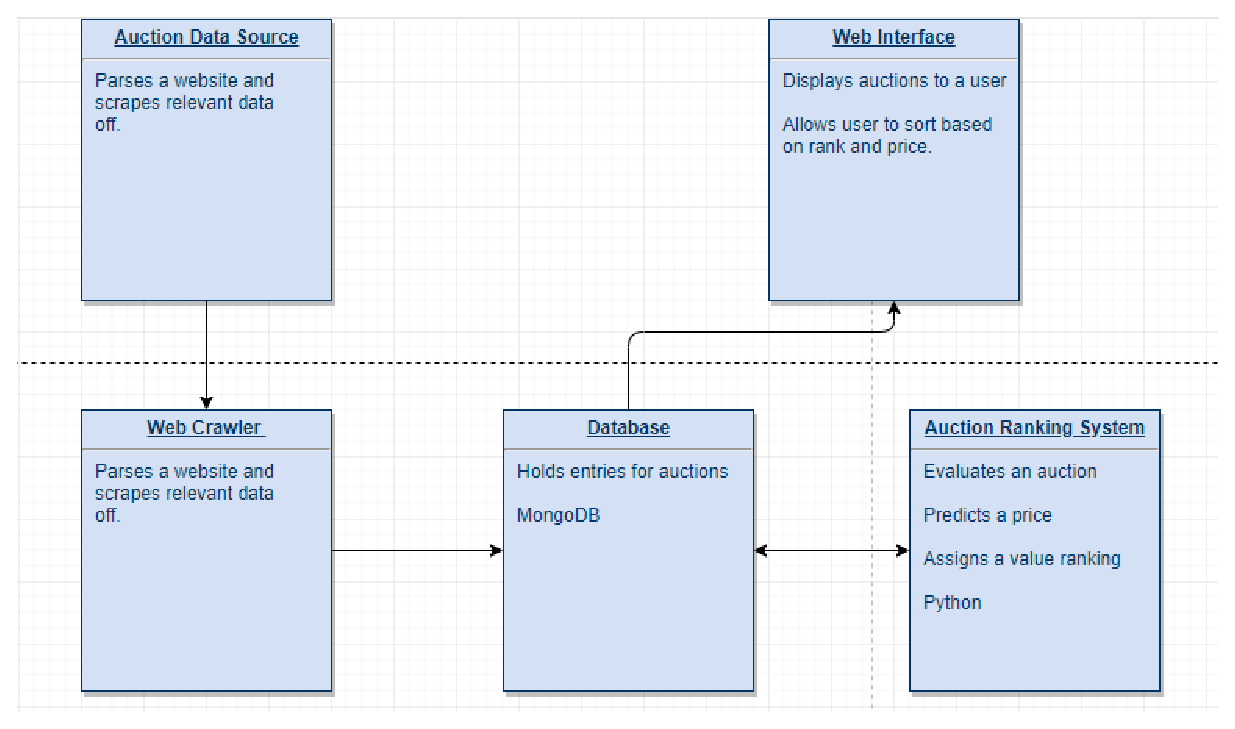
\includegraphics[scale=0.5]{flow_capture}
\caption{Flow Design}
\label{fig:flow}
\end{figure}
\end{frame}

\section{Implementation Components}

\subsection{MongoDB Database}

\begin{frame}[fragile=singleslide]{MongoDB Database}
\begin{itemize}
\setlength\itemsep{2em}
\item Web scraper includes MongoDB pipeline
\item Data is added directly to the database
\end{itemize}
\begin{figure}[ht]
\begin{minted}{python}
def open_spider(self, spider):
    self.client = pymongo.MongoClient(self.mongo_uri)
    self.db = self.client[self.mongo_db]

def process_item(self, item, spider):
    self.db[self.collection_name].insert_one(dict(item))
    return item
\end{minted}
\caption{Scrapy MongoDB pipeline}
\end{figure}
\end{frame}

\begin{frame}[fragile=singleslide]{Database entries}
Database entries in MongoDB:

\begin{figure}[H]
\centering
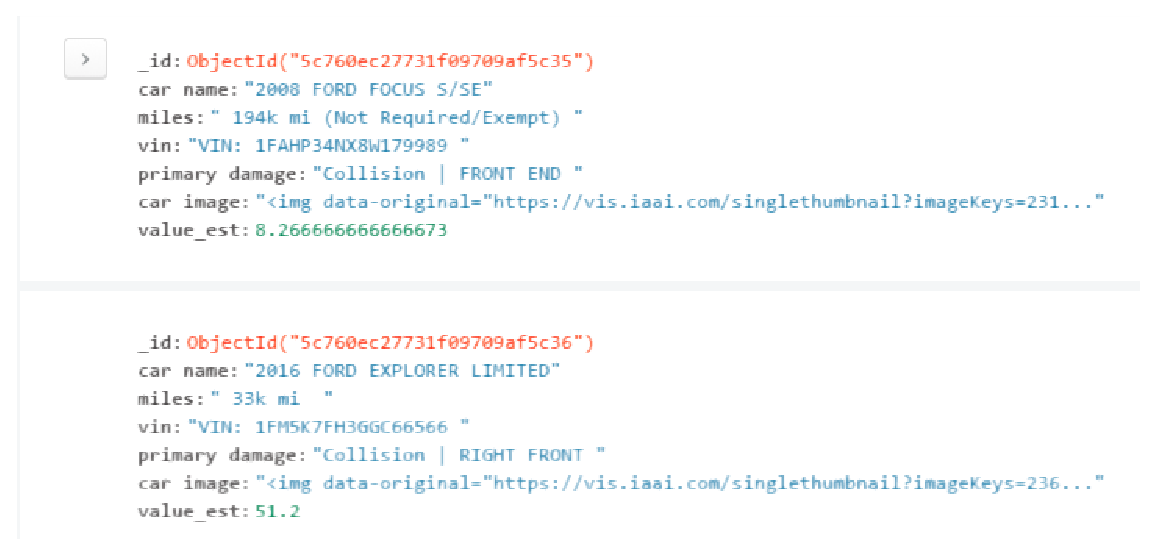
\includegraphics[scale=0.55]{db}
\caption{Database entries}
\label{fig:dbEntries}
\end{figure}
\end{frame}

\begin{frame}[fragile=singleslide]{Value Estimation}
\begin{itemize}
\setlength\itemsep{2em}
\item Naive value estimation based on damage and mileage
\item Certain attributes can be weighted
\item Will be improved as more data is available
\end{itemize}


\begin{minted}{python}
#Miles in thousands
value -= ((miles*2)/150.0 - 1)*self.milesWeight

#Damage from 0 to 5(most impactful damage) 
value -= damage*(self.damageWeight/2.0)
\end{minted}

\end{frame}

\subsection{Web Scraper}
\begin{frame}[fragile=singleslide]{Web Scraper}
\begin{itemize}
    \setlength\itemsep{2em}
    \item Users want to see the prices at different platforms at a single place.
    \item Some scrape examples
\end{itemize}

\begin{figure}[ht]
\centering

%is this still accurate?
\begin{minted}{python}
#create a basic spider "timedauctions"
scrapy genspider timedauctions
https://www.iaai.com/TimedAuctions
\end{minted}

\caption{Scrape Example}
\end{figure}

\end{frame}


\begin{frame}[fragile=singleslide]{Extracting Info}
\textbf{Extracting the URLs include salvage car photo:}
\begin{itemize}
    \item Using Google extension SelectorGadget. We found image's CSS labels are ".lazy".
\end{itemize}
\begin{figure}[ht]
\centering
\includegraphics[width=50mm]{salvagecarphoto}
\caption{Developer tools to find keys}
\label{fig:salvage}
\end{figure}
\begin{minted}{python}
#the CSS labels ".lazy" can extract image URLs. 
response.css(".lazy").extract()
\end{minted}
\end{frame}

\begin{frame}[fragile=singleslide]{Extracting Info}
\textbf{Extracting the URLs include salvage car vin:}
We can use a similar method to find VIN's location which is attributed of the  \textless tbody\textgreater  tag.

A screen shot is available on the next page.

\begin{figure}[ht]
\begin{itemize}
\begin{minted}{python}
response.css('a p:nth-child(3)::text').extract()
\end{minted}
\end{itemize}
\centering
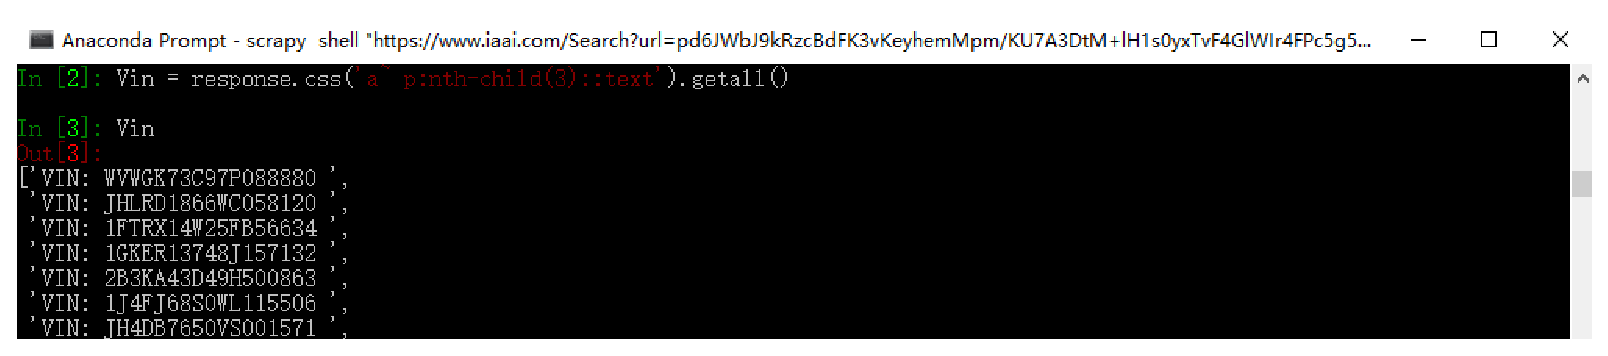
\includegraphics[width=100mm]{vinscrape}
\caption{Extract Example}
\end{figure}


\end{frame}

\begin{frame}[fragile=singleslide]{Extracting Info}
\textbf{Web Crawler Advancements}
\begin{itemize}
    \setlength\itemsep{2em}
    \item Getting the anchor element like"next" or "next page" to scrape all pages on specific website.
    \item Downloading extracted photos to local.
    \item Consolidating the extracted data of salvage car into database.
\end{itemize}
\begin{figure}[ht]

\label{fig:salvage2}
\end{figure}

\end{frame}


\subsection{Website Interface}

\begin{frame}[fragile=singleslide]{Web View}
\begin{figure}[h]
\centering
\includegraphics[scale=0.25]{HomePage}
\caption{HomePage of Auction Hunter}
\label{fig:homepage}
\end{figure}
\end{frame}

\begin{frame}{Website Interface}
\begin{itemize}
    \setlength\itemsep{2em}
    \item Backend written in Python using Django library
    \item Backend interacts with database to display data to user
    \item Frontend written in JavaScript using React framework
    \item Frontend uses Rest API to interact with the backend
\end{itemize}
\end{frame}

\begin{frame}[fragile=singleslide]{Web Code snippet}
\begin{figure}[H]
\begin{minted}{html}
return ( 
  <div><Grid container spacing={24}>
    {this.cars.map((car) => {
      return ( <Grid item xs={6}>
                 <AuctionCard
                   carImage={car.carImage}
                   carName={car.carName}
                   miles={car.miles}
                   vin={car.vin}
                   damage={car.damage}
                 />
               </Grid>
             )
         })} </Grid></div>); })
\end{minted}
\caption{web}
\end{figure}
\end{frame}

\begin{frame}[plain,c]
%\frametitle{A first slide}

\begin{center}
\Huge Demo
\end{center}

\end{frame}

\end{document}
